%!TEX root = ../dissertation.tex
\begin{savequote}[75mm]
``Before anything else, preparation is the key to success"
\qauthor{Alexander Graham Bell - Inventor}
\end{savequote}

\chapter{A11Y Guide}
In preperation for the main deliverable a deeper level of knowledge in the
accessibility space was required. To gain this knowledge and inline with my
`Share Everything' approach it was decided that an `Accessibility
training guide' would be produced here on referred to as `A11Y guide'. The idea
being that in producing a guide for others, oneself would have to be
knowledgable enough to produce good content.

\section{Preparation}
\subsection{Planning}
% TODO - Reference curve: http://www.wranx.com/ebbinghaus-and-the-forgetting-curve/

As researched by \citep{Ebbinghaus} in 1885 the forgetting curve demonstrates the
amount of knowledge remembered after a period of time. See Fig.~\ref{fig:ebbinghaus}
Repeating or revising the learning unsuprisingly results in the knowledge
stored in memory for longer.

\begin{figure}[H]
\centering
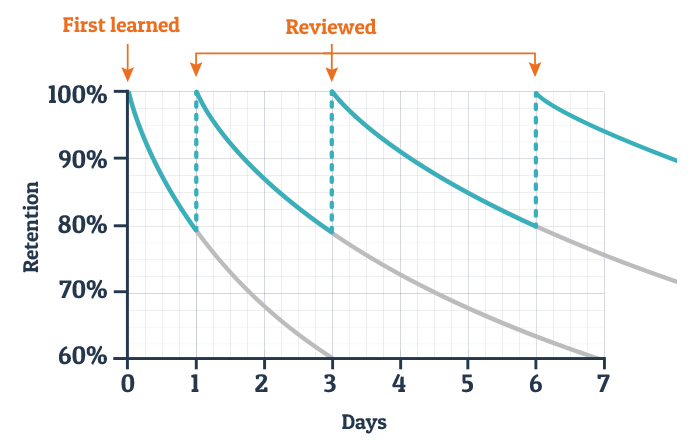
\includegraphics[width=0.5\textwidth]{figures/ebbinghaus}
\captionsetup{justification=centering}
\caption{Ebbinghaus' famous forgetting curve
\label{fig:ebbinghaus}}
\end{figure}

With this in mind I plan to iteratively build the A11Y Guide so
that the knowledge will be reinforced. The steps for its production will be
as follows:
\begin{enumerate}
  \item Search for useful resources online (First time learning)
  \item Score the identified resources with the assistive tools for a first hand
  experience along with other criteria (Second time repeating)
  \item Collate the resources under the correct header in a github project
  \item Setup continuous deployment scripts to ensure deploy on commit
  \item For each header create and document best practices (Third time
  repeating)
  \item Build a basic documentation website
  \item For each header create coded examples (Fourth time repeating)
\end{enumerate}

As explicitly stated there will be four loops of observing, reviewing and
applying the knowledge learned which should result in a peak in knowledge
when producing the tool.

\subsection{Building A11Y Guide Requirements}
In parallel to the above, for the guidance to have a greater impact it
needs to be current, relevant and available. This will require some additional
work to research the current direction the industry is moving and also the
requirements of Capgemini's teams.

\subsubsection{Understanding industry movement}
\label{sec:uim}
The purpose of understanding the current industry is to ensure that the
content within the guide is relevant and inline with the current status of the
industry. By understanding where the industry had come from and where it was
going would enable me to filter `old' resources from `new' resources and thus
produce more relevant guidance. See \ref{sec:GatheringKnowledge} for more
detail on the collection phase.

Being an apprentice within the industry I have exposure to general movements
and directions (through colleagues and self found sources), but primary
evidence was required to back up my personal opinion.

In 2016 the largest survey ever of front end developers was completed the
'State of JS' \citep{StateOfJs}. This survey covered almost every aspect of the front end
from javascript frameworks through tooling, all the way to testing frameworks.
Participants were asked to categorise technologies into the following five
pointers:
 \begin{itemize}
  \item `Used it before, would use again'
  \item `Used it before, would not use again'
  \item `Heard of it, would like to learn'
  \item `Heard of it, not interested'
  \item `Never heard of it'
 \end{itemize}

Based on my constant technology tracking I hypothesised that the technologies
that were `Used it before, would use again' and `Heard of it, would like to
learn' were the big winners in 2017. In Javscript frameworks this was ReactJs
and Angular 2. Again this needed clarification so I chose to use `Google
Trends' \citep{GoogleTrends} a tool which allows users to view graphs of
search queries on a
relative scale. During development most software engineers will
refer to google for documentation and issues so I felt this was going to be a
sound method for determining this. Fig.~\ref{fig:js_compare} confirms my
hypothesis and shows how ReactJS overtook AngularJS with Angular 2 on the rise.

\begin{figure}[H]
\centering
\centering
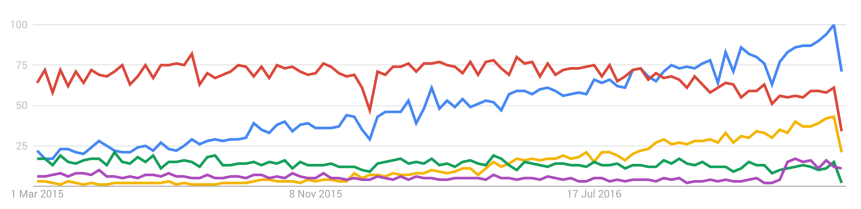
\includegraphics[width=\textwidth]{figures/js_compare}

\includegraphics[width=\textwidth]{figures/js_compare_key}
\captionsetup{justification=centering}
\caption{March 2017 Snapshot of JS Frameworks on Google Trends
\label{fig:js_compare}}
\end{figure}

\subsubsection{Questionnaire}
% TODO
% - Reference Professional competency scale https://hr.od.nih.gov/workingatnih/competencies/proficiencyscale.htm
% - Reference Remote working Capgemini
% - Reference google forms

The questionnaire's purpose is to understand the frameworks, components and
competencies in use across Capgemini. The next three paragraphs describe what
I want to discover and why.

The frameworks currently in use and those developers are competent in
\ref{fig:current_proj}, \ref{fig:competent_in}. These will be used to backup the hypothesis' made in
\label{sec:uim} and also enable me to feedback into my team on any gaps we
have within the industry.

Web Components client applications have in them \ref{q:5}. This will
determine the order in which guidance is generated in the A11Y Guide.
As I am aiming for continuous delivery, by adding the 'higher usage'
components first I will be adding value from the most valuable to the least
valuable.

The level of competency developers have in accessibility \ref{q:6}. This will
help understand the level at which to pitch the guidance (The target audience)
and will answer the question ``What level of competency can be assumed?". My
aim is to use the National Health competency scale \citep{NHComptency} to
asses this.

Google Forms was used to implement the questionnaire due to its simple
setup and integration into Google Spreadsheets which made the following
analysis much easier.

Out of a possible 69 team members 40\% (26 members) responded.

The first two questions showed how most software developers are using or are
competent in either React or AngularJS. This with the fact that
React was discovered as an upcoming technology in \ref{sec:uim} suggests the
examples in the A11Y guide should be written in React and library
recommendations made with this in mind. It is a fair assumption that
developers competent in React should be able to apply the knowledge learned
to Angular JS. Fig.~\ref{fig:current_proj} and Fig.~\ref{fig:competent_in}
are bar charts of the results given. A suprise discovery was the popularity
of JQuery. This is likely due to its widespread usage historically as it is
slowly becoming legacy.

\begin{figure}[H]
\centering
\centering
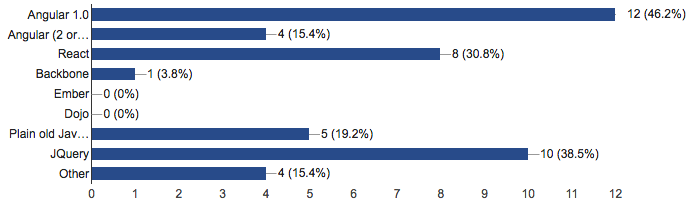
\includegraphics[width=\textwidth]{figures/questions/frameworks_in_use}
\captionsetup{justification=centering}
\caption{JS Frameworks Capgemini developers are using on current projects
\label{fig:current_proj}}
\end{figure}

\begin{figure}[H]
\centering
\centering
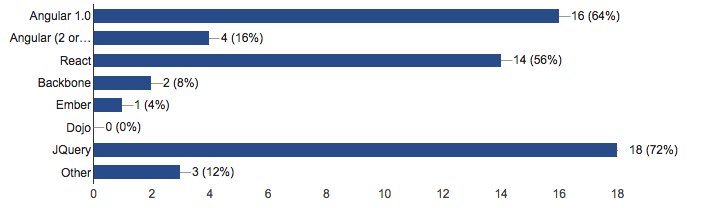
\includegraphics[width=\textwidth]{figures/questions/frameworks_competent_in}
\captionsetup{justification=centering}
\caption{JS Frameworks Capgemini developers consider themselves comfortable in
\label{fig:competent_in}}
\end{figure}

The next two questions focussed on understanding the software components in
use across client projects. An important aspect of many of our clients user base
is data entry and it is vital that users of assistive tools can interact and
understand these. The first question revolved around this and asked ``What
form components are in use on your current project?". The next question was
targeting more data consumption and higher level components so asked ``What
web components are in use on your project".

Unsuprisingly of the form components Fig.~\ref{fig:form_components}, textual
inputs (23/26 respondants) were the highest with select menus (22/26) and
validation messages (20/26) close behind. These would therefore be completed
first in the A11Y guide.

\begin{figure}[H]
\centering
\centering
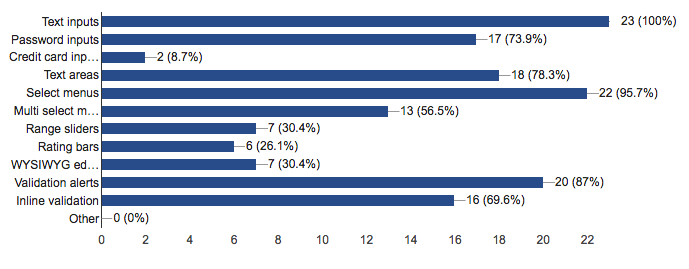
\includegraphics[width=\textwidth]{figures/questions/form_items}
\captionsetup{justification=centering}
\caption{Form components in use across Capgemini projects
\label{fig:form_components}}
\end{figure}

At a data consumption level there was a small anomoly in the data. `Images'
had accumulated 27/26 respondants. Due to the small sample size I dug into the
raw data and discovered that the `Images' option appeared twice on the
possible answers. With manual counting of this value, the correct number
of respondants was actually 17/26.

With images now normalised Navbars, Tabs, and Images all had 17/26 usages.
These were shortly followed by Dialogs (16/26) and Tables (16/26). Fig
.~\ref{fig:components_in_use} shows the full results.

\begin{figure}[H]
\centering
\centering
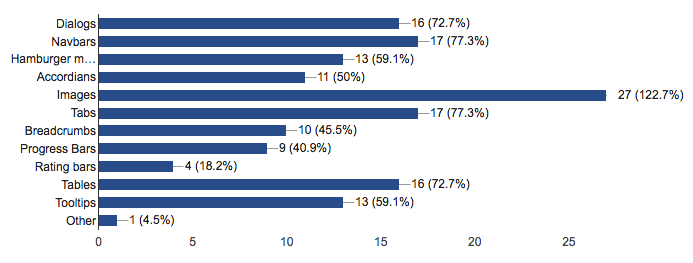
\includegraphics[width=\textwidth]{figures/questions/components_in_use}
\captionsetup{justification=centering}
\caption{Web components in use across Capgemini projects
\label{fig:components_in_use}}
\end{figure}

The final quesion asked each individual to rate themselves on the National
Health competency scale \citep{NHComptency}. I added some additional guidance
to the different levels to try and get a consistent answer across the
participants.
\begin{itemize}
\item None
\item Fundamental Awareness - Know what it is, but not how to implement it
\item Novice - Can implement with help from Google
\item Intermediate - Can implement with help and has experience testing with tools such as JAWS, Dragon
\item Advanced  - Can implement without help, understands \& explains how.
Knows best practice
\item Expert - The `go to' person for web accessibility
\end{itemize}

Due the questionnaire being anonymous it is a fair assumption that honest
answers are more probable. It is interesting how 18/26 ~70\% of respondants
have had no experience with the testing tools and rely upon Google to
understand accessibility. Fig.~\ref{fig:a11y_level} once again highlights
the requirement a project around accessibility is required at Capgemini.

\begin{figure}[H]
\centering
\centering
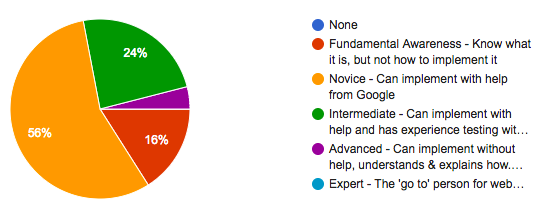
\includegraphics[width=\textwidth]{figures/questions/a11y_level}
\captionsetup{justification=centering}
\caption{Accessibility competency level across employees.
\label{fig:a11y_level}}
\end{figure}.

\subsection{Gathering Knowledge}
\label{sec:GatheringKnowledge}
This section will describe the methods and results of gathering resources to
be used to support the A11Y Guide.

\subsubsection{Method}
I chose to apply a method to ensure consistency and quality. The first and
simplest method I experimented with was to collate the top five results from
`Google'. This was the obvious and quickest method to gather such information
however, after reviewing resources in `Links' and `Buttons' items which I am
personally familiar with. I found a lot of overlap between content and after
testing them with the tools, similar mistakes across all of them.
None seemed to capture the `why' which naturally meant I needed a
different method.

To produce a new method I started by understanding what I needed to know to
produce the content. By understanding this I would be able to produce a method
by which I could assess an individual resources relevance and usefulness. The
key things I needed to know were:

\begin {itemize}
\item What does bad look like?
\item What do I need to do? e.g Coding Examples
\item Why should I write my code this way?
\item How do the assistive tools handle the outputs?
\item How can one test for correctness?
\end{itemize}

I produced 10 questions each with a possible score of 10. I was looking to
use the three best scoring resources in my content.

\subsubsection{Example Scoring}


\subsubsection{Outputs}
Inline with my `Open Source' and `Share Everything' ethos the resources were
sorted based upon their content and placed upon my github account in a public
 repository.
See Fig \ref{fig:allyLinksDemo}.
Following the principles of Continuous Delivery this could in fact be
considered the v1.0.0 of my A11Y Guide.

\begin{figure}[H]
\centering
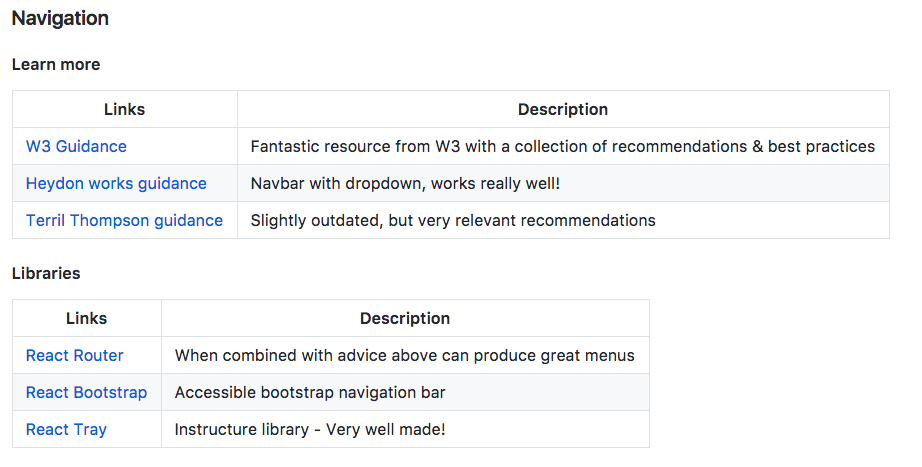
\includegraphics[width=\textwidth]{figures/documentation_link_example}
\captionsetup{justification=centering}
\caption{A demonstration of the `Navigation' content on Github.
https://github.com/Geeman201/a11y-links/
\label{fig:allyLinksDemo}}
\end{figure}


\subsubsection{Defining Requirements}
\label{sec:requirements}
From the questionnaire, common web frameworks, knowledge gained from the
resources and inline with my manifesto I started to write down concrete
requirements. I used \cite*{DanNorth}'s ``What's in a Story" method to write the
requirements. I find this method gives both `the what' and `the why' which
enables a better decision making process to be followed. As an additional
benefit in this format I have a solid means by which I can evaluate the
solution later.

\begin{center}
 \begin{tabular}{| c |}
 \hline
 As a developer \\
 \hline
 I want to have a section highlighting the most important aspects I need to
 take on board \\
 So that when I can quickly apply them on my current project \\
 \hline
 I want to have coded examples written in React \\
 So that I can understand and apply the knowledge \\
 \hline
 I want to have audio/subtitled examples of how the tools behave  \\
 So that I know the impact (The why) of Good/Bad semantics  \\
 \hline
 I want relevant links available  \\
 So that I can find more information out  \\
 \hline
\end{tabular}
\end{center}

\section{Deliverable}
% TODO -
% Reference Github - https://github.com/open-source
\subsection{Iteration 1 - Create content using markdown}
The first iteration of developing content was targetted the broader aspects
which affect every part of the users experience. This covered page structure,
page content and other general aspects like typography and colour. The content was produced
using Markdown \citep{Markdown}.

\subsubsection{Why Markdown?}
Markdown was chosen as it is fast becoming the `developer standard' for writing
documentation. When producing content, familiarity is key to producing an
enviornment in which people will collaborate. If you first have to
learn a new language or tool the barrier to entry to produce the content is
higher and thus you are less likely to do it. As Github the `worlds biggest'
\citep{GithubBig} software control platform has bought into markdown as way
developers communicate `most' developers have at least some knowledge in the
area. If they do not, the documentation for using markdown is well estabilished.

An additional benefit to using markdown is it is relatively difficult to make
the content you produce ``Inaccessible". As I want the guide to demonstrate
best practices; it should really be following them. Markdown compilers are
great at transforming content into `assistive tool' friendly HTML.

Fig \ref{fig:hierarchy} and Fig \ref{fig:structures} demonstrates how the
content is displayed in github's standard folder view. The markdown text is
converted into HTML and displayed in a clear well structured manner.

\begin{figure}[H]
    \centering
    \begin{subfigure}[b]{0.25\textwidth}
        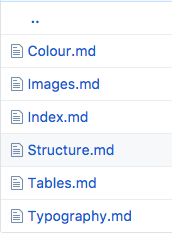
\includegraphics[width=\textwidth]{figures/documentation_md_example_1}
        \captionsetup{justification=centering}
        \caption{The File Hierarchy of `Content' section}
        \label{fig:hierarchy}
    \end{subfigure}
    \qquad
    %add desired spacing between images, e. g. ~, \quad, \qquad, \hfill
      %(or a blank line to force the subfigure onto a new line)
    \begin{subfigure}[b]{0.4\textwidth}
        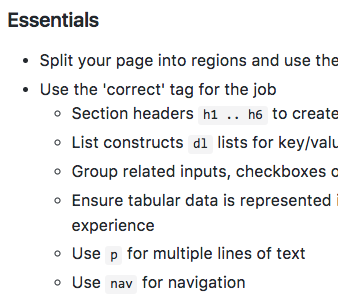
\includegraphics[width=\textwidth]{figures/documentation_md_example_2}
        \captionsetup{justification=centering}
        \caption{The `structures.md' file rendered in the browser}
        \label{fig:structures}
    \end{subfigure}
\end{figure}

\subsection{Iteration 2 - UI Design \& Build site}
This iteration focussed on taking the content I had produced and turning it
into an easily consumable website. Using this content and the requirements set
out in \ref{sec:requirements} the design would need to support:
\begin{itemize}
\item Coded Examples (Prefferably with snippet highlighting)
\item Snippets of the assistive tools reaction to good/bad markup
\item Navigation for a hierarchical structure
\item The best practices it describes
\end{itemize}

I chose to split the page into three sections as shown in Fig
.~\ref{fig:sections}. The first contained navigation. The second the main
content and coded examples. The third any 'additional information' such as
audio snippets and 'noteworthy' elements.

\begin{figure}[H]
\centering
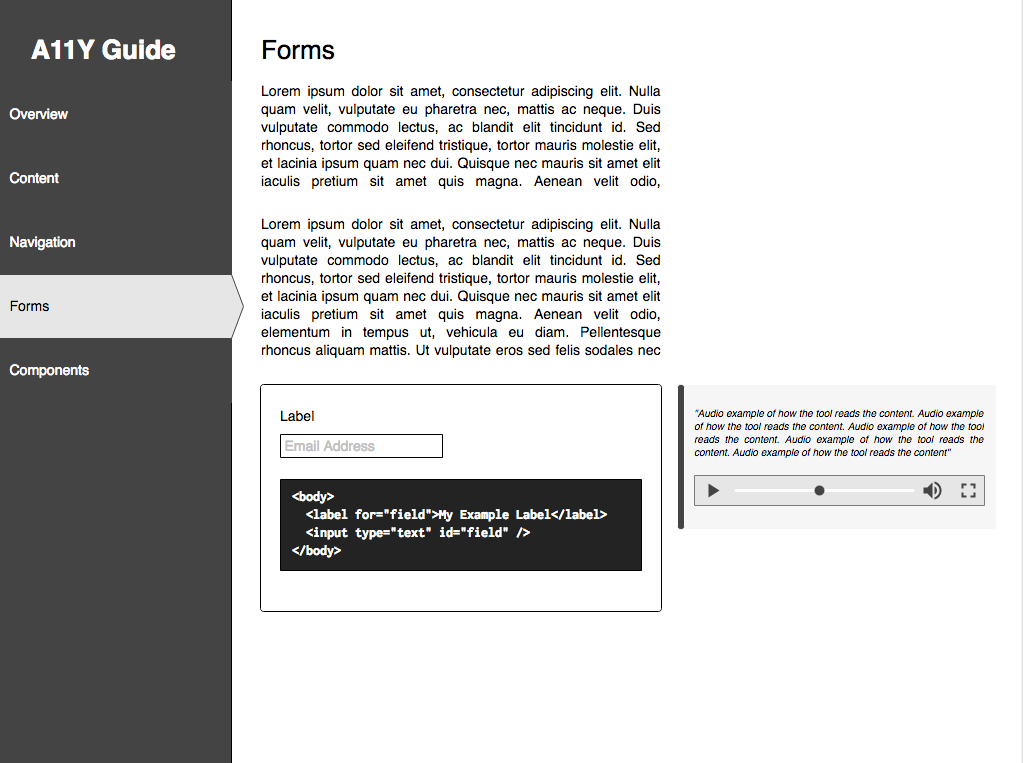
\includegraphics[width=0.9\textwidth]{figures/a11y_guide_design}
\captionsetup{justification=centering}
\caption{An example of the design built using \cite*{Moqups}
\label{fig:a11y_guide_design}}
\end{figure}

Using the content I had I produced a system design See Fig
.~\ref{fig:allycomponent}. As the content was held in markdown files the
documentation framework would have to parse the markdown and generate a
navbar and HTML. The idea was to enable the documentation framework to be
reused by abstracting the framework away from the content itself. For a user
of the documentation framework, I wanted them to only have to edit the
content and/or the Table of Contents. This would enable content to be the
users main focus and thus speed up the development of content for the guide.

\begin{figure}[H]
\centering
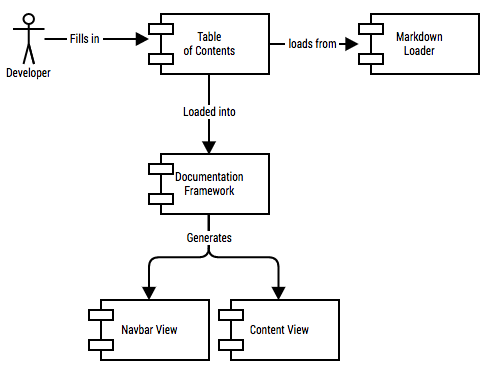
\includegraphics[width=0.65\textwidth]{figures/documentation_design}
\captionsetup{justification=centering}
\caption{Component Diagram for A11Y Guide
\label{fig:allycomponent}}
\end{figure}

A table of contents was
chosen rather than automatically loading folder structures so that users
could be in control of the ordering on the navbar. The table of contents
would be a JSON array with each object containing the following data:
\begin{itemize}
\item label - This would be the title of the page
\item url - This would be the path so content could be linked to directly
\item component - The markdown file to render
\item children - An array of children pages with the same JSON object structure.
\end{itemize}
A side effect of this design which was only realised in Iteration 4 was the
added benefit of extensibility and customisability of labels, url paths and
components. See Section \ref{sec:iteration_4} for how this design enabled custom
components to be used.

The web app was built using 'create-react-app' \citep{CreateReactApp} a tool
built by facebook for enabling the quick production of React web applications.
When the CLI tool runs it generates a basic web application with some sample
code. To reduce the risk later and following the continous delivery
guidelines \citep{ContinuousDelivery} I decided now was a good time to set up
my deploy pipeline. Fig.~\ref{fig:cd_pipeline} demonstrates the pipeline
through a sequence diagram.

\begin{figure}[H]
\centering
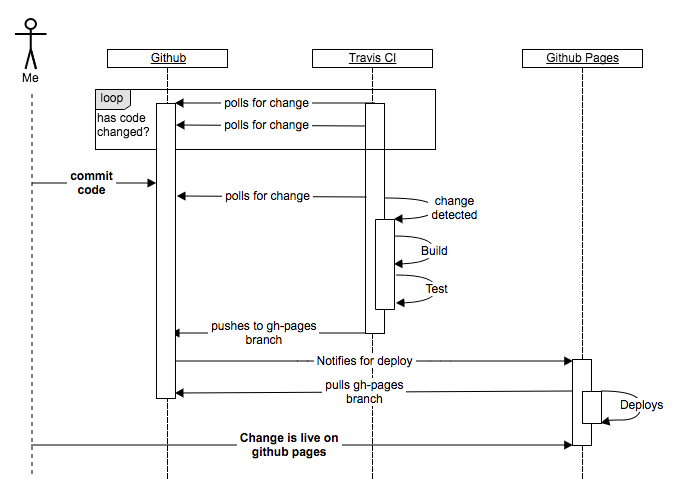
\includegraphics[width=0.7\textwidth]{figures/deploy_pipeline}
\captionsetup{justification=centering}
\caption{Upon Commit, the project is built/tested before being deployed to
Github Pages
\label{fig:cd_pipeline}}
\end{figure}

\subsection{Iteration 3 - Continue content}
As described by the title this iteration focussed on producing more content;
specifically around the forms and components identified in the questionnaire.
With the continuous deployment pipeline setup changes were instantly
consumeable at \url{https://geeman201.github.io/geemans-a11y-guide/}

\subsection{Iteration 4 - Recognise/Implement custom pages}
\label{sec:iteration_4}
When producing examples for dialogs and tabs the
need for the ability to insert very custom code surfaced. I was finding myself
hacking around in complex markdown which was difficult to understand. I decided
to alter the documentation framework to enable React Components to be injected.
How these slotted into the design is
shown in \ref{fig:allycomponent_2}. Note how the rest of the documentation
framework didn't have to change!

\begin{figure}[H]
\centering
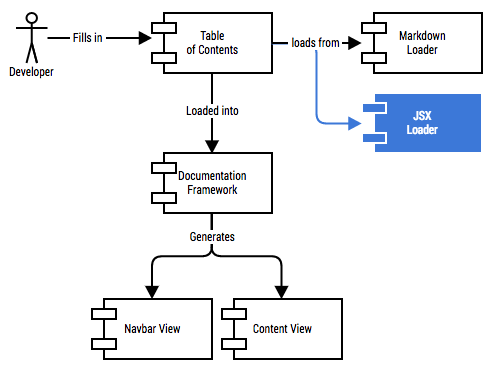
\includegraphics[width=0.65\textwidth]{figures/documentation_design_2}
\captionsetup{justification=centering}
\caption{Component Diagram for A11Y Guide with added JSX
component loader highlighted in blue.
\label{fig:allycomponent_2}}
\end{figure}

\subsection{Iteration 5 - Continue content}
This iteration involved returning to the pages which required custom
components. Dialogs and Tabs were completed and I also returned to the form
pages to add some additional examples.

\subsection{Iteration 6 - Generify}
This iteration focussed on extracting the common documentation framework that
had been produced. Removing the content and setting up a different repository
which others could clone and create their own documentation from.



%Principally, this chapter should describe the work that was undertaken before
%code was written, hardware built, theories worked on, or research studies
%executed. It should show how the project proposal was further refined and
%clarified, so that the implementation/research execution stage could go
%smoothly rather than by trial and error. This part of the report is attempting to
%prove that you went through a planning process before embarking on the
%deliverable so among others it might include discussion of:
%
%1. For software projects, a requirements analysis, HCI designs, architectural
%and use-case diagrams, etc.
%2. Any programming languages learnt, any complicated theories or algorithms
%that required understanding
%3. For research-based projects, the research approach (experimental design,
%where applicable), including methods and tools that were used/applied. If the
%research method involves the development of prototypic software to test a
%concept, briefly describe the design, structure, and creation of this software.
%Research methods should be described such that a third party could replicate
%the study/experiment to validate the results.
%
%This section should be answering the question “How did I plan to achieve the
%deliverable?”
